\subsection{Answer to Question \ref{q:why}}\label{subsec:why}
Building on Theorem \ref{thm:char}, we can now give a compelling
explanation to the measurement clusterization we observed for the
inverse problem of the heat equation, see Section
\ref{subsub:clusterization1} below. We also suggest a generic
explanation for clusterization, see Section \ref{subsub:clusterization2}.

\subsubsection{Clusterization in the heat equation}
Consider $\fwd$ and $\prcov$ from \emph{the inverse problem of the
heat equation}. As before, we denote the eigenvalues of
$\fwd\prcov\fwd^*$ by $\lambda_j$. We input these eigenvalues into our
\emph{generic} model, and find a D-optimal design $\opt$ for our
generic model using Theorem \ref{thm:char}. In our generic model, the
measurements we take are best utilized in reducing uncertainty for the
first $k$ eigenvectors. So, a D-optimal design arising from our
\emph{generic model} completely avoids measuring eigenvectors $k+1$
and above.

Of course, in a real life problem --- such as the inverse problem of
the 1D heat equation --- it is likely impossible to find measurement
locations for which all eigenvectors $k+1$ and above are
zero. However, if the eigenvalues of $\fwd\prcov\fwd^*$ decay quickly
(recall the square-exponential decay for eigenvalues of the 1D heat
equation in eq.\eqref{eq:decay}), a D-optimal design will try to
balance measuring a small number (i.e.~$k$) of the leading
eigenvectors.

The abovementioned balance is explored in
Fig.~\ref{fig:eigenvectors}. We allow $m=4$ measurements in $\Omega =
[0,1]$ and observe that D-optimal measurement locations are clustered
at $x_1 = 0.31$ and $x_2 = 0.69$. Upon close inspection of the scaled
eigenvectors of $\fwd \prcov \fwd^*$, we first observe that
eigenvectors $3$ and above have negligible prior amplitude. Since we
only have $m=4$ measurements at our disposal, we interpret these
results, following Theorem \ref{thm:char}, as implying we should only
care about measuring the first and second eigenvectors. Then, we note
the D-optimal $x_1,x_2$ present a compromise between the amplitude of
the first and second eigenvectors. For example, a measurement at
$x=0.5$ would have ignored the second eigenvector altogether, since
the second eigenvector is zero at $x=0.5$.

Now we can understand measurement clusterization for the inverse
problem of the heat equation. A D-optimal design attempts to measure
the first $k$ eigenvectors of $\fwd \prcov \fwd^*$. But there may be
(spatial) limitations on where these $k$ eigenvectors have large
amplitude. For the inverse problem of the heat equation there are two
spatial locations that present a good compromise between the
amplitudes of the first and second eigenvectors, namely $x_1$ and
$x_2$ --- see Fig.~\ref{fig:eigenvectors}. We have $m=4$ measurements
at our disposal but only two spatial locations that are a good
compromise between the first and second scaled eigenvectors. Thus,
clusterization arises as a consequence of the pigeonhole principle.

\begin{figure}\label{fig:eigenvectors}
    \centering
    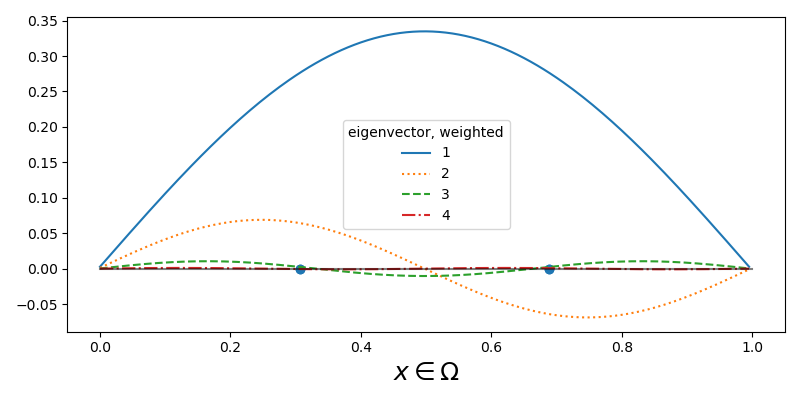
\includegraphics[width=\textwidth]{figs/eigenvectors_dst_scaled.png}
    \caption{D-optimal measurement locations ($m=4$ measurements) and
      weighted eigenvectors for finding the initial condition of the
      1D heat equation. Measurement locations and weighted
      eigenvectors are plotted over the computational domain $\Omega =
      [0, 1]$ (x-axis). Measurement clusterization occurs
      approximately at $0.31$ and $0.69$. These two locations are a
      compromise between the magnitudes of the first and second
      eigenvectors, which are the eigenvectors that a D-optimal design
      aims to measure. Allocating $m=4$ measurements into two
      locations results in clusterization, according to the pigeonhole
      principle.}
  \label{fig:why}
\end{figure}
